Given a time horizon $T$, the amount of fish extracted for the end of this time, is given by
\begin{equation}
	J(u;T)=\int_{0}^{T} u(t)\diff{t}
\end{equation}
Where $u(t)$ is the harvesting rate at time $t$, introduced to the population as follows,
\begin{equation}
	\dev{x}{t}=rx\left(1-\frac{x}{M}\right)-u(t) \label{eq: HarvestOpenLoop}
\end{equation}
We would like to know among all the possible time functions $u\in \mathbb{R}^{[0,T]}$, the functional $J$ is maximized. 

Stating in this way, is not well posed. Since we see that the functional is linear in $u$, implying the bigger gets $u$, the bigger gets $J$. But this approach has the disadvantage we showed in the previous discussion, that the bigger $u$ the fastest our population can lead to extinction and therefore, we will not be able to continue harvesting the pool. 

From the previous results we see that for $u(t)>\frac{rM}{4}$, we lead the population to extinction. Therefore, we restrict our harvesting rate $u$ to,
\begin{equation}
0\leq u(t)\leq\frac{rM}{4}. \label{eq: OpenLoopConstrain}
\end{equation}

Please note that, the equation \ref{eq: HarvestOpenLoop} can be rewritten in this way,
\begin{equation}
	u(t)=rx\left(1-\frac{x}{M}\right)-\dev{x}{t} \label{eq: OpenLoopControl}
\end{equation}
and the functional $J$ now, as a map of $x$ and $\dot{x}=\dev{x}{t}$ instead of $u$.
\begin{equation}
	J(x,\dot{x};T,r,M)=\int_{0}^{T} \left(rx\left(1-\frac{x}{M}\right)-\dot{x}\right) \diff{t} \label{eq: Functional for Population.}
\end{equation}
We can restate the problem as follows, we would like to find the population $x(t)$ among all the possible populations\footnote{We see from equation \ref{eq: Functional for Population.}, that the space where we are trying to find the optimum is $\LL([0,T])\cap \mathrm{BV}([0,T])$, where $\mathrm{BV}(\Omega)$ is the space of bounded variations over some open set $\Omega$. }, such that $J$ is maximized. Once we know the population, we can construct a control $u(t)$ such that equation \ref{eq: HarvestOpenLoop} is satisfied. Then, we ask the condition for $x \in C^1([0,T])$.

Therefore, the pair $x^*$, $\dot{x}^*$ that maximizes the functional $J=\int_0^T L(x, \dot{x}, t)\diff{t}$, should satisfy the Euler-Lagrange equations,

\begin{equation}
	\dev{}{t}\left(\pdev{L}{\dot{x}^*}\right)-\pdev{L}{x^*}=0
\end{equation}

where $L:[0,T]\times C^1([0,T]) \mapsto \mathbb{R}$. In our case $L(x,\dot{x}, t)=u(t)$, as stated in equation \ref{eq: OpenLoopControl}. Therefore,

\begin{align}
	\dev{}{t}\left(\pdev{u}{\dot{x}^*}\right)-\pdev{u}{x^*}&=0 \nonumber\\ \dev{}{t}\left(1\right)-r+2r\frac{x}{M}&=0 \nonumber\\
	\implies x- \frac{M}{2}&=0
\end{align}

Hence $J$ has one stationary point $x^*(t)=\frac{M}{2}$. Moreover, $L$ is concave for the pair $(x, \dot{x})$, therefore the function $x^*(t)$ is a maximum, and is unique. 

From equation \ref{eq: HarvestOpenLoop}, when $x^*(t)=\frac{M}{2}$ we need to construct the control $u(t)$, as follows,
\begin{equation}
	u(t)=r\frac{M}{2}\left(1-\frac{x}{M}\right)=\frac{rM}{4}
\end{equation}

We observe that, when $x(t)=x^*(t)$, the control is the maximum of the constrain \ref{eq: OpenLoopConstrain}, we have imposed from the analysis of the fixed points of the dynamic. 

Knowing the fact, that most of the times the initial population is not always $\frac{M}{2}$, we implement the following harvesting strategy.

\begin{equation}
	u(t)=\begin{cases}
	0 & x(t)<x^*(t) \\
	\frac{rM}{4} & x(t)=x^*(t) \\
	\omega>\frac{rM}{4} & x(t)>x^*(t)
	\end{cases}
\end{equation}
Where $\omega$ is some rate a bit greater than $rM/4$, fixed according to the requirements of the implementation. The aim of this strategy is to approach the fastest as possible to the stationary point of $J$. This can be seen as a raw closed loop dynamic, since our control is a function of the population $x$, as explained in the section \ref{sec: ClosedLoop}.

\subsection{Noise Effect.}
Even we obtained a result for the optimum for $J$, realistically, this is a bad harvesting strategy, since we are considering the controls and the populations ideal. And small deviations in the dynamic.

In order to have a better understanding of the reality, we add the effect of noise to the dynamic.


Consider the presence of white noise, normally distributed, added in multiplicative way to the population. That is the higher the population we have, the noise increases proportional. Then, we can write the logistic equation under the optimal harvesting rate as a Weiner process,
\begin{equation}
dx=\left(rx\left(1-\frac{x}{M}\right)-\frac{rM}{4}\right)\diff{t}+\sigma x\diff{W} \label{eq: Constant Harvesting Stochastic Control}
\end{equation}
Figure \ref{fig: NoiseIdealConstant} shows a simulation of the behavior of the ideal dynamic under the presence of noise with $\sigma=0.1$.

\begin{figure}[H]	
	\begin{center}
	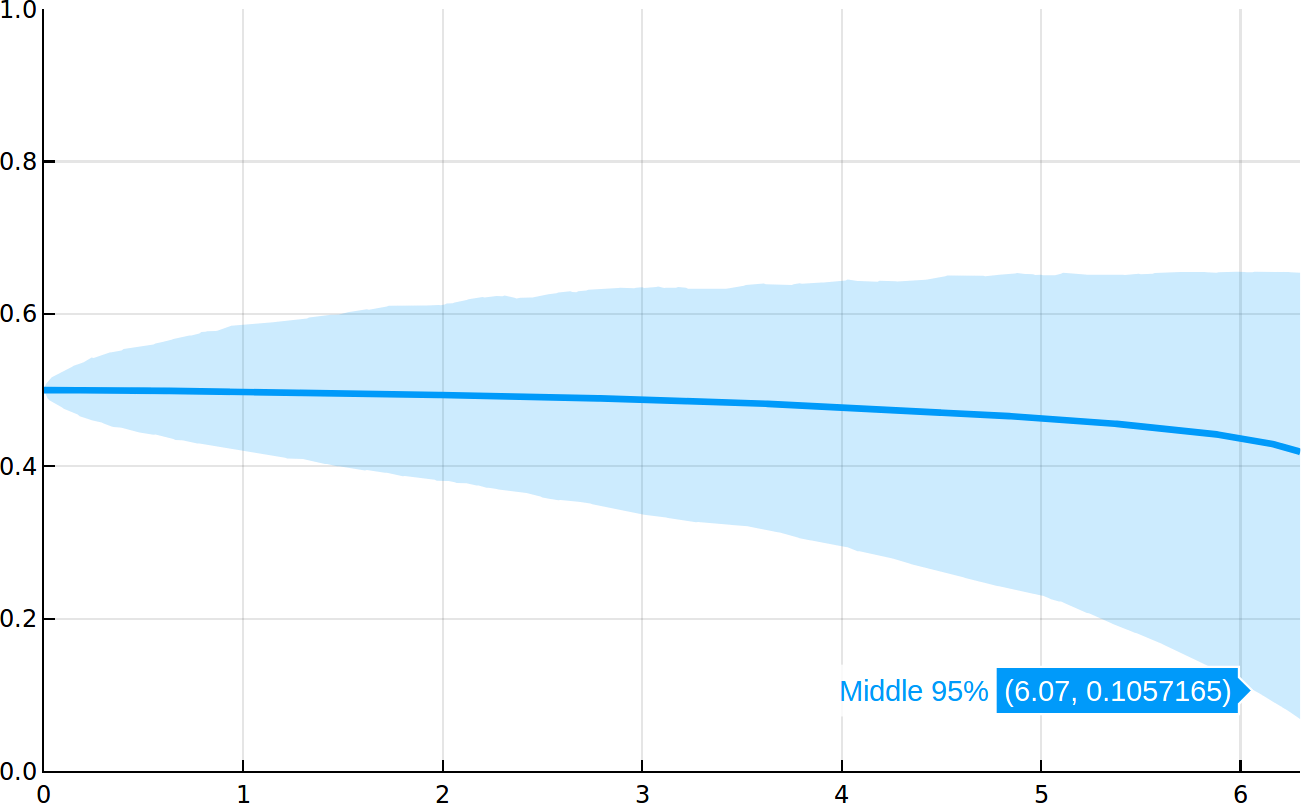
\includegraphics[width=0.5\textwidth]{NoiseIdealDynamic.png}
	\caption{Ideal Optimum $x^*$ under presence of noise. Population in $M$-units of  and time in units of $r$-units.}
	\label{fig: NoiseIdealConstant}
	\end{center}
\end{figure}

We can interpret figure \ref{fig: NoiseIdealConstant}, as follows, with probability 0.95, our dynamic will lie in the space covered by the light blue area, with median shown by the darker line. What is really bad, since we can appreciate we have the probability to lead our population to extinction. Moreover, we can see from the graphic that for approximately six $r$ units our population will descend from $0.5M$ to around $0.4M$ in the middle situation and will decrease to around $0.1M$ in a bad situation.

In addition to the discussion, figure \ref{fig: NoiseIdealConstant2} shows the $95\%$ and $50\%$ quantiles for the dynamic, (blue and orange area respectively).

\begin{figure}[H]
	\begin{center}
		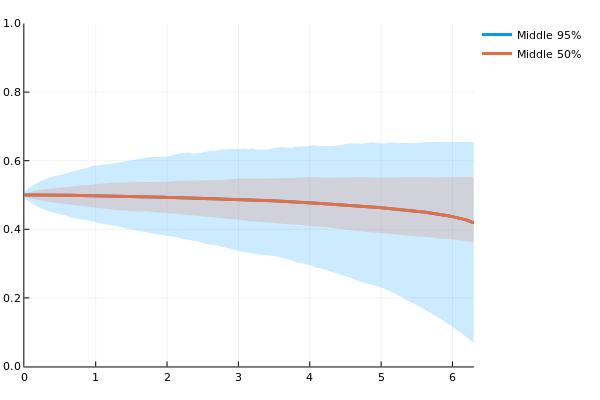
\includegraphics[width=0.5\textwidth]{NoiseIdealDynamic2.png}
		\caption{Quantiles for the ideal dynamic.}
		\label{fig: NoiseIdealConstant2}
	\end{center}
\end{figure}

Our suggestion is to use a smarter constant harvest rate: $\bar{u}<u^*$, but close to the dynamic of $(x^*,u^*)$.
 
Since this for $u<u^*$ generates two fixed points, with one of them stable, most probably will not decreases until extinction. Moreover, in a really bad case it will decrease to the unstable fixed point. Also note that the middle dynamic will increase to the stable fixed point. 

We show the following results for $u=0.9u^*=\frac{9}{40}rM$ and time horizon of six $r$-units. 

\begin{figure}[H]
	\caption{Noise Tolerant Harvesting.}
	\begin{center}
		\begin{subfigure}{0.3\textwidth}
			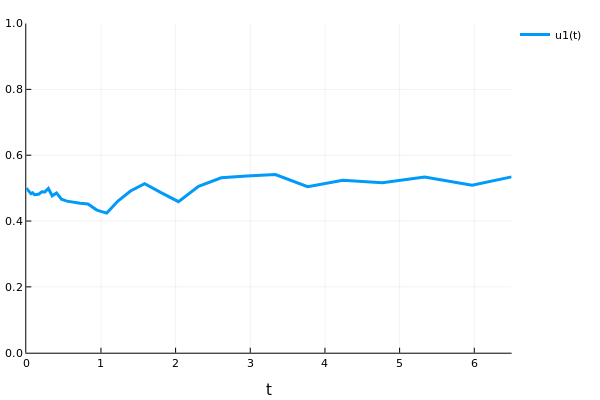
\includegraphics[width=0.95\textwidth]{NoisePresenceDynamic.png}
			\caption{One simulation performed of the dynamic for $\bar{u}=0.9u^*$.}
		\end{subfigure}
		\begin{subfigure}{0.3\textwidth}
		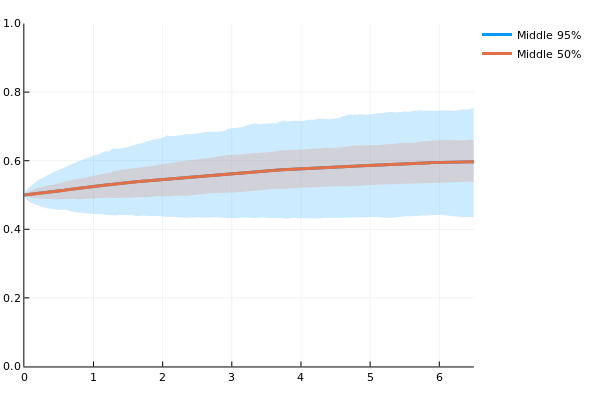
\includegraphics[width=0.95\textwidth]{SmarterNoiseTolerant2.png}
		\caption{0.95 and 0.5 quantiles}
		\end{subfigure}
		\begin{subfigure}{0.3\textwidth}
			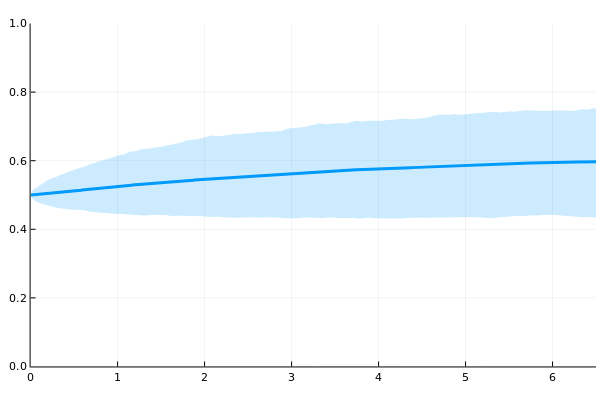
\includegraphics[width=0.95\textwidth]{SmarterNoiseTolerant.png}
			\caption{0.95 quantile}
		\end{subfigure}
	\end{center}
\end{figure}